% Charlotte Geiger - Manuel Lippert - Leonard Schatt
% Physikalisches Praktikum

% Main-Datei für die Auswertung in TeX

% Struktur:
% Für jeden Abschnitt gibt es einen Ordner, damit jeder individuell an seinen Aufgaben arbeiten
% kann, ohne beim merge in GitHub Konflikte zu erhalten. Deshalb werden alle Unteraufgaben auch 
% extra in Ordner angelegt. Die einzelnen Dateien über den input Befehl einfügbar.
% Bilder und andere Grafik werden im Ordner Grafik abgelegt 


% Packages
\documentclass[paper=a4,bibliography=totoc,BCOR=10mm,twoside,numbers=noenddot,fontsize=11pt]{scrreprt}
\usepackage[ngerman]{babel}
%\usepackage[babel,german=quotes]{csquotes} %For Quotes
\usepackage[T1]{fontenc}
\usepackage[latin1, utf8]{inputenc}
\usepackage{lmodern}
\usepackage{graphicx}
\usepackage{nicefrac}
\usepackage{fancyvrb}
\usepackage{amsmath,amssymb,amstext}
\usepackage{siunitx}
\usepackage{url}
\usepackage{natbib}
\usepackage{microtype}
\usepackage[format=plain]{caption}
\usepackage{physics}
\usepackage{titleref}

% Zusätzliche Packages
\usepackage{geometry}
\usepackage{anyfontsize}
\usepackage[table]{xcolor}
\usepackage{ifthen}
\usepackage[absolute,overlay]{textpos}
\usepackage{amsfonts}
\usepackage{xstring}
\usepackage{tikz}
\usepackage{pdfpages}
\usepackage{booktabs}
\usepackage{hyperref}
\usepackage{minibox}

% Abschnittseinrückung und -abstand
% Die folgenden Zeilen sollen möglichst nicht verändert werden
\parindent 0.0cm
\parskip 0.8ex plus 0.5ex minus 0.5ex

% Anzahl und Größe von Gleitobjekten
% maximal 2 Objekte oben und unten
% erlaubt auch größere Bilder, welche die ganze Seite benötigen
% Die folgenden Zeilen sollen möglichst nicht verändert werden
\setcounter{bottomnumber}{2}
\setcounter{topnumber}{2}
\renewcommand{\bottomfraction}{1.}
\renewcommand{\topfraction}{1.}
\renewcommand{\textfraction}{0.}

%\sc und \bc veraltet. Daher: (20.09.2018)
\DeclareOldFontCommand{\sc}{\normalfont\scshape}{\@nomath\sc}
\DeclareOldFontCommand{\bf}{\normalfont\scshape}{\textbf}

% Verschiedenes
\pagestyle{headings}          % Der Seitenstil sollte möglichst nicht verändert werden
\graphicspath{{./bilder/}}    % Der Pfad für die Abbildungen Abbildungen wird gesetzt
\VerbatimFootnotes            % \verb etc. auch in \footnotes mφglich

% Funktionen
\newcommand\tab[1][1cm]{\hspace*{#1}}
\newcommand{\vect}[1]{\boldsymbol{\mathbf{#1}}}
\newcolumntype{g}{>{\columncolor[rgb]{ .741,  .843,  .933}}l}
% Tiefgestellte Zahlen nicht kursiv
\catcode`_=\active
\newcommand_[1]{\ensuremath{\sb{\mathrm{#1}}}}

\begin{document}

    \nonfrenchspacing

    % 0. Kapitel Cover
    % Manuel Lippert - Paul Schwanitz
% Physikalisches Praktikum

% 0. Cover
% Noch abänderbar nur ein Vorschlag
\newgeometry{top=30mm, bottom=20mm, inner=20mm, outer=20mm}
\thispagestyle{empty}

% Colors
\definecolor{Notablue}{HTML}{3498DB}		%Theoretische Physik
\definecolor{Notared}{HTML}{CF366C}			%Mathematik
\definecolor{Notagreen}{HTML}{19B092}		%Experimentalphysik
\definecolor{Notaorange}{HTML}{FA9D00}		%Chemie/Wahlfach nicht physikalisch
\definecolor{Notagrey}{HTML}{969696}		%Praktikum
\definecolor{Notalavendel}{HTML}{9DBBD8}	%Wahlfächer physikalisch

% Boolean by default false
\newboolean{twoRows}
\newboolean{symbol}

% Funktions
\makeatletter
   \def\vhrulefill#1{\leavevmode\leaders\hrule\@height#1\hfill \kern\z@}
\makeatother
\newcommand*\ruleline[1]{\par\noindent\raisebox{.8ex}{\makebox[\linewidth]{\vhrulefill{\linethickness}\hspace{1ex}\raisebox{-.8ex}{#1}\hspace{1ex}\vhrulefill{\linethickness}}}}

% Variables
\def\schriftgrosse{40}
\def\linethickness{1,5pt}

\def\farbe{black}
\def\fach{PPBphys2}
\def\name{Manuel Lippert - Paul Schwanitz}
\def\uberschrift{Chaos in einfachen \\[0,5cm] physikalischen Systemen} % Absatz mit \\[0,5cm]; u = Übung, k = Klausur; s = Skript, e = Ergebnis
\def\bottom{WS2021/22}
\def\datum{06.09.2021}
\def\platz{B11 | 0.09}
\def\betreuer{Reinhard Richter}

\def\teilnehmerm{Manuel Lippert}
\def\emailm{Manuel.Lippert@uni-bayreuth.de}
\def\teilnehmerp{Paul Schwanitz}
\def\emailp{Paul.Schwanitz@uni-bayreuth.de}

%\def\auswertp{}
%\def\messp{}
%\def\protop{}

\def\groupnr{11}

\begin{titlepage}
			
	\centering
	{\LARGE \sffamily {\textbf{\bottom}\par}}
	\vspace{2,5cm}
    {\fontsize{30}{0}\sffamily\ruleline{\textcolor{\farbe}{\textbf{\fach}}}\par}
    \vspace{6cm}
	{\Large\sffamily \ruleline{\name}\par}
	
	
	% Choose Text
	\ifthenelse{\equal{\uberschrift}{s}} {\def\titel{Skript}}	
		{\ifthenelse{\equal{\uberschrift}{k}} {\def\titel{Klausur}}
			{\ifthenelse{\equal{\uberschrift}{u}} {\def\titel{Übung}}
				{\ifthenelse{\equal{\uberschrift}{e}} {\def\titel{Klausur \\[0,5cm] Ergebnis}}
					{\def\titel{\uberschrift}}
				}
			}
		}
	
	\IfSubStr {\titel} {\\[0,5cm]} {\setboolean{twoRows}{true}} {\setboolean{twoRows}{false}}
	
	\ifthenelse{\boolean{twoRows}}
		{
			\begin{textblock*}{21cm}(0cm,8,5cm) % {block width} (coords), centered		
				{\fontsize{\schriftgrosse}{0}\sffamily\textcolor{\farbe}{\textbf{\titel}}\par}
			\end{textblock*}
		}
		{
			\begin{textblock*}{21cm}(0cm,9cm) % {block width} (coords), centered		
				{\fontsize{\schriftgrosse}{0}\sffamily\textcolor{\farbe}{\textbf{\titel}}\par}
			\end{textblock*} 
		}
	
	% Choose Logo
	\ifthenelse {\equal{\farbe}{Notared}} {\def\logo{Bilder/Logo/UniBTNotared}}
		{\ifthenelse {\equal{\farbe}{Notagreen}} {\def\logo{Bilder/Logo/UniBTNotagreen}}
			{\ifthenelse {\equal{\farbe}{Notablue}} {\def\logo{Bilder/Logo/UniBTNotablue}}
				{\ifthenelse {\equal{\farbe}{Notaorange}} {\def\logo{Bilder/Logo/UniBTNotaorange}}
					{\ifthenelse {\equal{\farbe}{Notagrey}} {\def\logo{Bilder/Logo/UniBTNotagrey}}
						{\ifthenelse {\equal{\farbe}{Notalavendel}} {\def\logo{Bilder/Logo/UniBTNotalavendel}}	
							{\ifthenelse {\equal{\farbe}{black}} {\def\logo{Bilder/Logo/UniBT}}	
								{\def\logo{noLogo}}
							}
						}
					}
				}
			}
		}	

	\IfSubStr{\logo}{noLogo}{\setboolean{symbol}{false}}{\setboolean{symbol}{true}}
	
	% Gruppe
	\vspace{10cm}
	{\large\sffamily{Gruppe \groupnr}}
	
	%Logo
	\vfill

	\ifthenelse{\boolean{symbol}}
		{
			\begin{figure}[h]
			\begin{center}
				
				\includegraphics[width=2cm]{\logo}
				
			\end{center}
			\end{figure}
		}
	
\end{titlepage}

\restoregeometry

% Information
\chapter*{Informationen}
\label{chap:info}

\begin{tabular}{l l}

	{\textbf{Versuchstag}} \hspace{1cm} & \hspace{1cm} {\datum}\\[0,2cm]
	{\textbf{Versuchsplatz}} \hspace{1cm} & \hspace{1cm} {\platz}\\[0,2cm]
	{\textbf{Betreuer}} \hspace{1cm} & \hspace{1cm} {\betreuer}\\[1,2cm]
	{\textbf{Gruppen Nr.}} \hspace{1cm} & \hspace{1cm} {\groupnr}\\[0.2cm]
	{\textbf{Teilnehmer}} \hspace{1cm} & \hspace{1cm} {\teilnehmerm}\\[0.2cm]
						  \hspace{1cm} & \hspace{1cm} {\emailm}\\[0.2cm]
						  \hspace{1cm} & \hspace{1cm} {\teilnehmerp}\\[0.2cm]
						  \hspace{1cm} & \hspace{1cm} {\emailp}\\[0.2cm]

	%{\textbf{Auswertperson}} \hspace{1cm} & \hspace{1cm} {\auswertp}\\[0.2cm]
	%{\textbf{Messperson}} \hspace{1cm} & \hspace{1cm} {\messp}\\[0.2cm]
	%{\textbf{Protokollperson}} \hspace{1cm} & \hspace{1cm} {\protop}\\[0.2cm]

\end{tabular}

    \thispagestyle{empty}
    \cleardoublepage
    \tableofcontents
    \cleardoublepage

    % 1. Kapitel Einleitung
    %Matteo Kumar - Leonard Schatt
% Fortgeschrittenes Physikalisches Praktikum

% 1. Kapitel Einleitung

\chapter{Einleitung}
\label{chap:einleitung}

Radioaktivität ist ein uns immer umgebender Umweltfaktor. Dabei ist sie - neben den gesundheitlichen Schäden, die sie verursachen 
kann - oft ein nützliches Hilfsmittel. Sie kann zu medizinischen Zwecken eingesetzt werden, oder zur Materialanalyse. 
Dabei sind vor allem Alpha- und Gammastrahlung für die Identifikation von Materialien wichtig. Da diese diskrete und charakteristische 
Spektren haben, kann man mit diesen bestimmte radioaktive Isotope nachweisen. Dies werden wir in diesem Versuch durchführen. Des Weiteren 
verwenden wir die Strahlung zur Schichtdickenmessung. Insgesamt erhöht der Versuch die Kompetenzen im Umgang mit radioaktiven Präparaten und 
macht sensibler für die damit verbundenen Gefahren.


    % 2.Kapitel Fragen zur Vorbereitung
    % Charlotte Geiger - Manuel Lippert - Leonard Schatt
% Physikalisches Praktikum

% 2.Kapitel Fragen zur Vorbereitung

\chapter{Fragen zur Vorbereitung}
\label{chap:fvz}

% <<<<<<< TO DO'S:
% - Fazit
% - FzV3: Skizzen für $n_2<n_1$ und für $n_1<n_2$
% - FzV6: Polardiagramme aus unterer Quelle einfügen

%1
\section{Allgemeines}

\subsection*{Polarisation durch Reflexion}
Bei Auftreffen von unpolarisiertem Licht - zum Beispiel von einer Glühbirne oder von der Sonne - auf eine Glasplatte teilt sich das Licht in einen reflektierten und einen gebrochenen Lichtstrahl auf. 
Der reflektierte Strahl ist  linear polarisiert, wenn der Winkel zwischen reflektiertem in gebrochenem Strahl dem Brewster-Winkel entspricht. Dieser beträgt 90 Grad. Ist diese Voraussetzung nicht erfüllt, so entsteht nur teilweise Polarisation. 
\footnote{\url{http://www.chemgapedia.de/vsengine/vlu/vsc/de/ph/14/ep/einfuehrung/wellenoptik/polarisation_b.vlu.html}}

\subsection*{Polarisation durch Brechung und Doppelbrechung}
Eine Möglichkeit für die Polarisation durch Brechung ist bei Eintritt von Lichtstrahlen in bestimmte Kristalle, beispielsweise Quarze. Licht wird hierauf je nach seiner Schwingungsrichtung in verschiedener Weise gebrochen, sind aber immer linear polarisiert. 
Kristalle weisen die Eigenschaft auf, dass sie in unterschiedliche Richtungen unterschiedlich das Licht brechen. Dieses Verhalten nennt man optisch anisotrop. Bei solchen Materialien tritt Doppelbrechung auf. Aber auch bei optisch isotropen Medien (beispielsweise Glas oder Wasser) kann Doppelbrechung vorkommen. Dieses Phänomen ist  bei Verformung des Materials durch Zug- und/oder Druckkräfte zu beobachten, was man als Spannungsdoppelbrechung bezeichnet. 
\footnote{\url{https://www.lernhelfer.de/schuelerlexikon/physik-abitur/artikel/polarisation-von-licht-durch-reflexion-und-brechung}}
\newpage
\subsection*{Polarisation durch Streuung}
Auch durch Streuung kann polarisiertes Licht erzeugt werden. Je nach Polarisationsrichtung wird Licht an einem sogenannten Streuzentrum unterschiedlich stark in unterschiedliche Richtungen gestreut. Das Streuzentrum ist beispielsweise ein Atom oder ein Molekül. Fällt unpolarisiertes Licht auf solch ein Streuzentrum, so wird es angeregt und das Licht wird gestreut. Da die Streurichtung ungleich der Einfallsrichtung ist, so kann man folgendes Phänomen erkennen:  Das in y-Richtung gestreute Licht wird vollständig linear in z-Richtung, das in z-Richtung abgestrahlte Licht in y-Richtung polarisiert. Daher erkennt man in bestimmten Raumrichtungen linear polarisiertes Licht.
\footnote{\url{https://www.leifiphysik.de/optik/polarisation/ausblick/polarisation-durch-streuung}}

\subsection*{Funktionsweise von Polarisationsfiltern}
Die Filter bestehen aus langen, parallel ausgerichteten Kettenmolekülen. Durch das Eintreten von unpolarisiertem Licht werden die Kettenmoleküle durch die dazu parallelen elektromagnetischen Wellen angeregt, wodurch die Welle absorbiert wird. Die zu den Kettenmolekülen senkrecht schwingende Wellen können die Moleküle nicht anregen, wodurch nur parallele Wellen absorbiert werden. Daher filtern Polarisationsfilter nur Licht bestimmter Polarisationsrichtung aus. 
Bei senkrechter Verdrehung von zwei identischen Polarisationsfiltern erkennt man eine deutliche Verdunklung, da dadurch zwei senkrecht zueinander stehende Wellen absorbiert wurden. 
\footnote{\url{https://www.leifiphysik.de/optik/polarisation/grundwissen/polarisation-von-licht-einfuehrung}}

\subsection*{Definition Polarisationsgrad}
Der Polarisationsgrad entspricht dem Verhältnis der Intensität des polarisierten Lichtanteils zur Gesamtintensität des Lichtes.
\footnote{\url{https://www.spektrum.de/lexikon/optik/polarisationsgrad/2622}}
\newpage
%2
\section{Zusammenhang von Intensität und elektrischem Feld}
Intensität wird in der Physik die Größe genannt, die die Flächenleistungsdichte beim senkrecht zur Ausbreitungsrichtung zeigende Transport von Energie beschreibt. 
Die Intensität wird im Versuch durch eine Photodiode gemessen. 
\begin{equation}
I=c\epsilon_0 E^2
\end{equation}
Mit dem elektrischen Feld E, beschrieben durch eine zeitlich periodische Funktion mit der Amplitude: $E=\sqrt{E_{\parallel}^2 +E^2_{\perp}}$, der Intensität $I=\frac{\epsilon_0\epsilon_mc_0}{2n_m}E^2$ und Medium m.
Gemessen wird das zeitliche Mittel der Intensität I
\footnote{Demtroder S. 188, 7.6}

%3
\section{Fresnel'sche Formeln für  Spezialfälle }
\subsection*{$\varphi=0\rightarrow\psi=0$}
Für die Fresnelschen Formeln gilt:
\begin{align*}
\frac{E_{r,\parallel}}{E_{e,\parallel}}=\frac{n_2-n_1}{n_2+n_1}\\
\frac{E_{t,\parallel}}{E_{e,\parallel}}=\frac{2n_1}{n_2+n_1}\\
\frac{E_{r,\perp}}{E_{e,\perp}}=\frac{n_1-n_2}{n_2+n_1}\\
\frac{E_{t,\perp}}{E_{e,\perp}}=\frac{2n_1}{n_2+n_1}\\
\end{align*}
Betragsmäßig unterscheiden sich die senkrechte und parallele Richtung des reflektierten und transmittierten Anteil bezüglich des Einfallsstrahls nicht und verhalten sich gleich. Der Grund dafür ist, dass die rotationssymmetrische Aufbauweise keine Vorzugsrichtung aufweist. \\
Nun betrachten wir die Energieerhaltung, die über folgende Formeln gegeben ist:
\begin{align*}
E_{r,\parallel}+\frac{n_2}{n_1}E_{t,\parallel}=E_{e,\parallel}\\
E_{r,\perp}+\frac{n_2}{n_1}E_{t,\perp}=E_{e,\perp}\\
\end{align*}
Der Faktor $\frac{n_2}{n_1}$ wird durch den Medienwechsel notwendig. Zu erkennen ist nun, dass der reflektierte Anteil steigt, je größer der Unterschied zwischen den Brechindices ist. \\
Bei mit betrachten des Winkels, muss man den Faktor $\frac{n_2}{n_1}$  um den Faktor $\frac{cos\psi}{cos\varphi}$ erweitern. 
Beide Richtungen der Polarisation verhalten sich gleich, wodurch man feststellt, dass sich durch senkrechten Durchgang keine Polarisationsgradänderung ergibt bzw. diese nicht möglich ist. Dadurch folgt: $P=const$

\subsection*{Brewster Gesetz und Brewsterflächen}
Das Brewster Gesetz lässt sich aus der Abstrahlcharakteristik der atomaren Dipole und dem snelliusschen Brechungsgesetz herleiten. Für die Herleitung wird meist angenommen, dass der  Strahl von dem Medium Luft mit Brechindex $n_1=1$ auf ein Medium aus einem anderer Material mit Brechindex $n_2$ fällt.\\
Die Definition des Brewster-Winkels lautet wie in Frage zur Vorbereitung 1 schon beschrieben folgendermaßen:
\begin{equation}
Theta_1=\Theta_b\Theta_2=90^o-\Theta_B
\end{equation}
Das Reflexionsgesetz besagt, dass Einfallswinkel $|Theta_1$ gleich Reflexionswinkel $\Theta_a$ sein muss. 
Eingesetzt in die das snelliussche Brechungsgesetz: 
\begin{equation}
n_1sin(\Theta_1)=n_2sin(\Theta_2)
\end{equation}
folgt nach umstellen das Brewstersche Gesetz:
\begin{equation}
n_1sin(\Theta_B)=n_2sin(90^o-\Theta_B)=n_2cos(\Theta_B) \tab \rightarrow \tab n_1=arctan(\frac{n_2}{n_1})
\end{equation}

\subsection*{$\varphi+\psi=\frac{\pi}{2}$}
Nun betrachten wir den Sonderfall des Brewsterwinkel. Damit gilt mit den trigonometrischen Umformungen $sin(\psi)=cos(\varphi)$ und analog $sin(\varphi)=cos(\psi)$:
\begin{gather*}
\frac{E_{r,\parallel}}{E_{e,\parallel}}=\frac{n_2cos(\varphi)-n_1sin(\varphi)}{n_2cos(\varphi)+n_1sin(\varphi)}= \frac{n_2cos(\varphi)-n_2cos(\varphi)}{2n_2cos(\varphi)}=0\\
\frac{E_{r,\perp}}{E_{e,\perp}}=\frac{n_1cos(\varphi)-n_2sin(\varphi)}{n_2cos(\varphi)+n_1sin(\varphi)}=\frac{n_1-\frac{n_2^2}{n_1}}{n_1+\frac{n_2^2}{n_1}}=\frac{n_1^2-n_2^2}{n_1^2+n_2^2}\\
\frac{E_{t,\parallel}}{E_{e,\parallel}}=\frac{2n_1cos(\varphi)}{2n_2cos(\varphi)}=\frac{n_1}{n_2}\\
\frac{E_{t,\perp}}{E_{e,\perp}}=\frac{2n_1cos(\varphi)}{n_2sin(\varphi)+n_1cos(\varphi)}=\frac{2n^2_1}{n_2^2+n_1^2}
\end{gather*}
Man sieht aus den Ergebnissen, dass der parallele Anteil komplett transmittiert und überhaupt gar nicht reflektiert wird. Daher ist der reflektierte Strahl komplett polarisiert. Somit gilt: $P_r=1$. Das ist auch die Besonderheit bei Brewsterwinkeln, dass der reflektierte Lichtstrahl senkrecht zur Einfallsebene polarisiert ist. \\
Dieses Phänomen wird viel in der Physik genutzt. Beispielsweise im Laser findet es Anwendung. Das sogenannte Brewster-Fenster funktioniert durch parallel zur Einfallslinie polarisierten Lichtfall, der durch eine im Brewsterwinkel zum Licht stehende Glasplatte bzw. einen Lichtkristall, fällt. Somit wird der Polarisationsgrad gesteigert, ohne die Intensität zu schwächen.  
\footnote{\url{https://www.geothermie.de/bibliothek/lexikon-der-geothermie/b/brewsterwinkel-brewstergesetz.html}}
\footnote{\url{http://www.techniklexikon.net/d/brewster-fenster/brewster-fenster.htm}}
\footnote{\url{https://de.wikipedia.org/wiki/Fresnelsche_Formeln}}
\begin{center}
    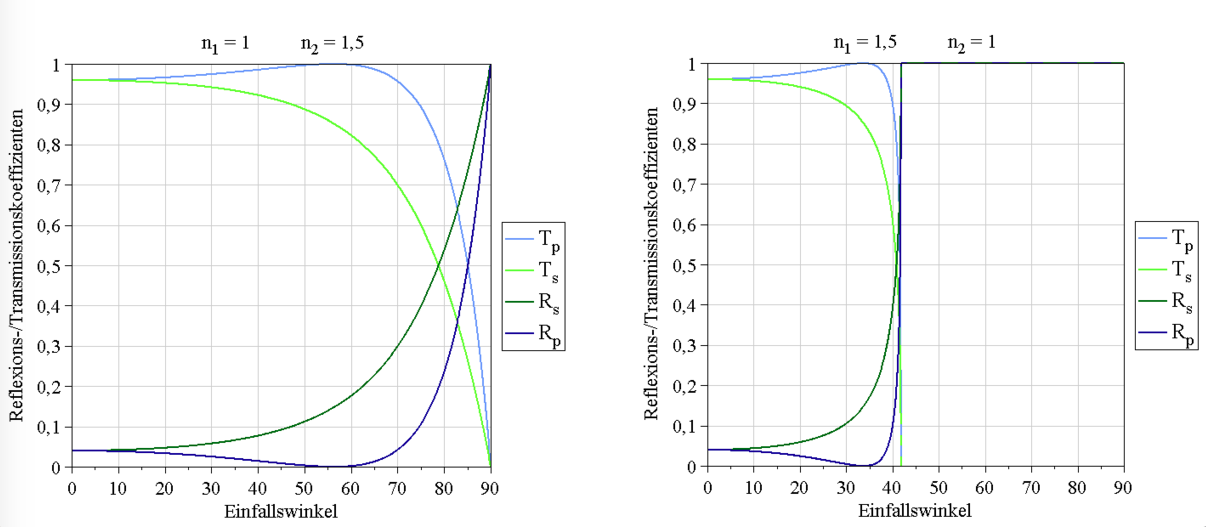
\includegraphics[scale=0.3]{Fresnelsche-Formeln2}
    \captionof{figure}{Reflexions-/Transmissionsvermögen R,T  für die Grenzfläche Luft n=1 und Glas n=1,5. Auf Grenzfläche einfallendes Licht von der Luftseite (=Seite des niedrigeren Brechungsindex) (links) und von der Glasseite (=Seite des höheren Brechungsindex) (rechts)}
\end{center}
%Subtitle: Reflexions-/Transmissionsvermögen R,T  für die Grenzfläche Luft n=1 und Glas n=1,5. Auf Grenzfläche einfallendes Licht von der Luftseite (=Seite des niedrigeren Brechungsindex) (links) und von der Glasseite (=Seite des höheren Brechungsindex) (rechts). 

%4
\section{ Intensität der Streustrahlung}
Für die Rayleigh-Streuung muss man sich zuerst der Schwingungseigenschaft von Luftmolekülen auseinandersetzen. Wie oben schon angedeutet können Moleküle nur in bestimmte Richtungen schwingen. Bei Anregung von Luftmolekülen entstehen induzierte elektrische Dipolschwingungen, die sogenannten Hertzschen Dipole. 
Die zur Polarisationsrichtung im Abstand r abgestrahlte Feldstärke kann man folgendermaßen berechnen:
\begin{equation}
E=\frac{\omega^2p}{4pi\varepsilon_0c^2r}
\end{equation}
mit Frequenz $\omega$ des abgestrahlten Lichts\\
Anzahldichte der Moleküle: N\\
E-Feldvektor des angeregten Lichts: $E_{in}=E_0sin(\omega t)$\\
Polarisation: P = $(\varepsilon_r-1)\cdot\varepsilon_0E_{in}$\\
Induzierter Dipolmoment des Moleküls: $p=\frac{P}{N}=\frac{\varepsilon_r-1}{N}\cdot\varepsilon_0E_{in}$\\
Gestreute Intensität (von Volumen mit N Molekülen): I$=\sim NV\cdot\overline{E^2}$\\
$I_{in}\sim\overline{E_{in}}$, $\omega=\frac{2pic}{\lambda}$, $\varepsilon_r=n^2$, $\overline{E^2_{in}=\frac{E_0^2}{2}}$  \\\\
\begin{equation}
\frac{I}{I_{in}}=\frac{NV\overline{E^2}}{S^2_{in}}=\frac{\pi^2V(n^2-1)sin^2(\vartheta)}{Nr\lambda^4}
\end{equation}
Dadurch erkennt man, dass die Intensität indirekt proportional zur vierten Potenz der Wellenlänge ist. Je größer die Wellenlänge, desto kleiner die abgestrahlte Intensität. Da Blau eine kleine Wellenlänge hat von ca. 400 nm, so ist die abgestrahlte Intensität deutlich gößer, als beispielsweise rot mit der Wellenlänge von 700nm.  Daher erscheint der Himmel blau. 
\footnote{\url{https://home.uni-leipzig.de/pwm/teaching/ExPhys3_WS0809/script/EP3_jan22_09.pdf}}

%5
\section{Winkelabhängigkeit der Rayleigh-Streustrahlung}
Die Lichtstreuung beruht allgemein darauf, dass durch die Lichtwelle im Dipole mit Ausrichtung in Polarisationsrichtung des Lichtes induziert werden. Die induzierten Dipole wiederum strahlen ein Lichtfeld der gleichen Frequenz ab. Die theoretische Winkelabhängigkeit der Streuintensität in der Streuebene ist je nach Polarisation des anregenden Lichts durch das Rayleigh-Gesetz vorgegeben. 
Nun diskutieren wir die Winkelabhängigkeit der Intensität der Rayleigh Streustrahlung anhand von Gleichung (7): 
\begin{equation}
    \text{Intensität} = S(\delta)=AIsin^2(\delta)
\end{equation}\
Mit der Quelle Demtröder S.321 der 7.Auflage folgt folgender Zusammenhang:
\begin{equation}
\overline{P_S}=N\sigma_S \overline{I}
\end{equation}
$\overline{P_S}$ als Streuleistung, $A=N\sigma(\omega)$ als Frequenzabhängigkeit, $\sigma$ als Streuquerschnitt und $\delta$ als betrachteter Winkel.\\
Daraus folgt:
\begin{equation}
I=I_0 sin^2(\delta)
\end{equation}
Dadurch wird deutlich, dass der Winkel $\delta$ je nach Polarisationsrichtung variiert. \\
Nun wird die Abhängigkeit der Polarisationsrichtung zur Streuebene betrachtet. 
Zuerst die Parallele Richtung:
%Bild 1 einfügen mit Polarisation parallel zur Streuebene
Aus der Abbildung erkennt man die geometrischen Zusammenhänge von $\delta=\frac{\pi}{2}-\Theta$. Damit folgt:
\begin{equation}
I(\Theta)=I_{0,\shortparallel}\cdot sin^2 (\frac{\pi}{2}-\Theta)=I_{0,\shortparallel}\cdot cos^2(\Theta)
\end{equation}
\begin{equation}
\Rightarrow S_{0,\shortparallel}\cdot cos^2(\Theta)
\end{equation}
Nun betrachten wir die senkrechte Polarisationsrichtung im Bezug zur Streuebene
%Bild 1 einfügen mit Polarisation senkrecht zur Streuebene
Aus dieser Abbildung kann man sehen, dass $\delta$ für jedes $\Theta$ immer $\frac{\pi}{2}$ bleibt. Damit folgt:
\begin{equation}
I(\delta=\frac{\pi}{2}) = I_{0,\perp}
\end{equation}
\begin{equation}
\Rightarrow S_\perp (\Theta) \sim AI_{0,\perp}
\end{equation}
Man erkennt, dass die Folgerungen (parallel, bzw senkrecht) den Gleichungen Gl. 8 und Gl.9 im Skript entsprechen. 
Durch die Szstem-Symmetrie haben Rückwerts- und Vorwärtsstreuung die gleichen Werte.
\footnote{\url{www.spektrum.de/lexikon/optik/rayleigh-streuung/2774}}

%6
\section{Starke Vorwärtsstreuung bei der Miestreuung}
Bei Lichtstreuung an festen Mikropartikeln beispielsweise Staub oder Rauch erkennt man eine elastische, kohärente Streuung. Diese Streuung von Licht an Teilchen mit einem ähnlich großen Durchmesser wie die Wellenlänge nennt man Mie-Lorentz Streuung. Die Intensität der Mie Streuung ist proportional zum quadrierten Durchmesser des streuenden Teilchens. Die gesamte gestreute Lichtintensität berechnet sich dann folgendermaßen:
\begin{equation}
I\propto \biggl| \sum_{K=1}^N A^2_K \biggl|
\end{equation}
$A_K$ ist die Streuamplitude des K-ten Moleküls im Partikel mit N Molekülen
Zustandekommen der starken Vorwärtsstreuung der Miestrahlung:\\
Für die Veranschaulichung der Mie-Streuung kann folgendes System betrachtet werden:\\
\begin{center}
    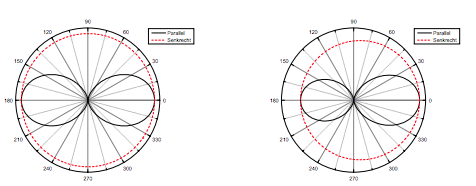
\includegraphics[scale=0.8]{Mie-Strahlung-Winkelverteilung}
    \captionof{figure}{Normiere Winkelverteilung des Streulichtes eines Tropfens mit einem Durchmesser von 0,01 µm (links) und 0,1 µm (rechts) mit beiden Polarisationsrichtungen}
\end{center}
%Untertitel des Bildes: Normiere Winkelverteilung des Streulichtes eines Tropfens mit einem Durchmesser von 0,01 µm (links) und 0,1 µm (rechts) mit beiden Polarisationsrichtungen.
Durch geometrische Überlegungen werden folgende Zusammenhänge deutlich:
\begin{align*}
\Delta_{vor}=\mid d-dcos(\Theta)\mid=d\mid 1-cos(\Theta) \mid\\
\Delta_{rück}=\mid d+dcos(\pi-\Theta_r)\mid=d\mid 1-cos(\Theta_r) \mid\\
\rightarrow \Delta = d\mid 1-cos(\Theta) \mid
\end{align*}
Der Phasenversatz ist also eine Funktion von $1-cos(\Theta)$.
Man erkennt, dass man durch diese theoretische Vorüberlegung keinen Unterschied zwischen Vorwärts und Rückwärts-Streurichtung ausmachen kann. \\
Bei den bisherigen Überlegungen haben wir den Abstand d als konstant angenommen. Dies gilt jedoch nur in der Theorie, da sich Teilchen in der Theorie durch thermische Bewegungen bzw. Schwingungen immer bewegen und sich so der Abstand dauerhaft verändert. Dies ist einer der Gründe, weshalb die Miestrahlung vor allem nach vorne streut. 
Für die "wirkliche" Beschreibung der starken Vorwärtsstreuung der Miestrahlung und anderer Effekte bei Streuung an Partikeln nutzt man die relativ komplizierte Lorenz-Mie-Theorie. Diese Theorie ist eine mathematisch genaue Beschreibung verschiedenster Streuphänomene von elektromagnetischer Wellen an Teilchen und die genaue Lösung der Maxwell-Gleichungen für die Streuung einer ebenen elektromagnetischen Welle an einem beliebig großen Teilchen. Jedoch wird für die Streuung an kleinen Teilchen $\lambda\gg D$ meist die unkompliziertere Berechnung der Rayleigh Streuung genutzt, obwohl auch die Mie-Theorie dies abdeckt. Es werden durch die Mie-Theorie Lösungen gefunden, die verschiedene Geometrien und Formen haben (ähnlich zu den Legendre - Polynomen der Quantenmechanik). Diese Formen zeigen, dass die Vorwärtsstreuung meist größer ist, als die Rückwärtsstreuung.
\footnote{\url{https://physik.cosmos-indirekt.de/Physik-Schule/Mie-Streuung}}
\footnote{Demtröder, Auflage 7, Kapitel 10.9.3, S.322}
\footnote{\url{http://webdoc.sub.gwdg.de/ebook/diss/2003/fu-berlin/1998/13/kap3.pdf}}

    % 3.Kapitel Protokoll
    % Charlotte Geiger - Manuel Lippert - Leonard Schatt
% Physikalisches Praktikum

% 3.Kapitel  Protokoll

% Variables
\def\skalierung{0.65}

\chapter{Messprotokoll}
\label{chap:protokoll}

Das Messprotokoll wurde am Versuchstag handschriftlich erstellt und hier als
PDF-Datei eingefügt. 

\section*{Zusatz}
Zusätzlich fügen wir die Bilder und die verwendeten Schaltungen des Versuchs nch dem Protokoll an zur besseren Übersicht.

% Einbindung des Protokolls als pdf (mit Seitenzahl etc.)
% Erste Seite mit Überschrift
%\includepdf[pages = 1, landscape = false, nup = 1x1, scale = \skalierung , pagecommand={\thispagestyle{empty}\chapter{Protokoll}}]
%            {03-Protokoll/Protokoll.pdf}
% Restliche Seiten richtig skaliert
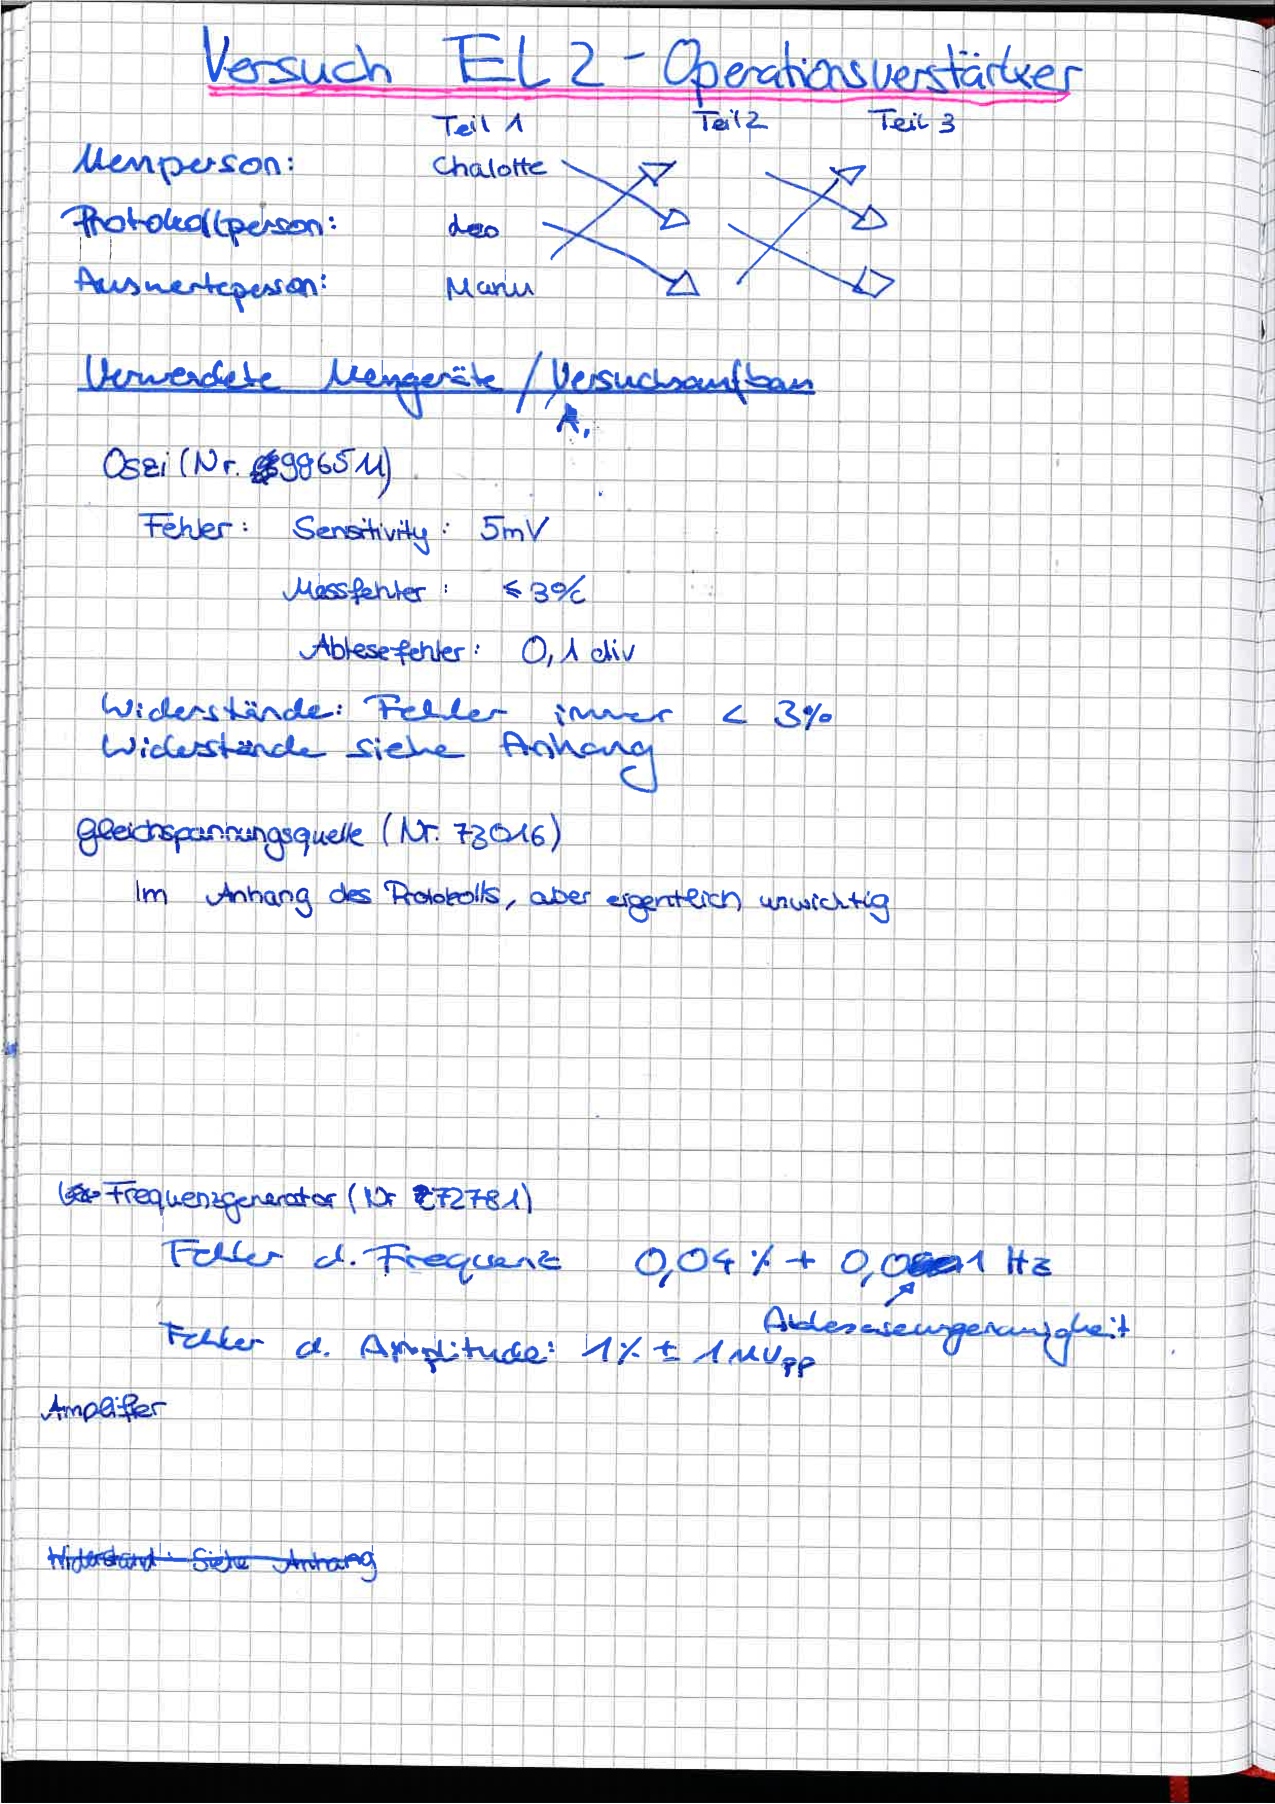
\includepdf[pages = -, landscape = false, nup = 1x1, scale = \skalierung , pagecommand={}]{30-ProtokollEL2.pdf}

%\section*{Steckbretter}
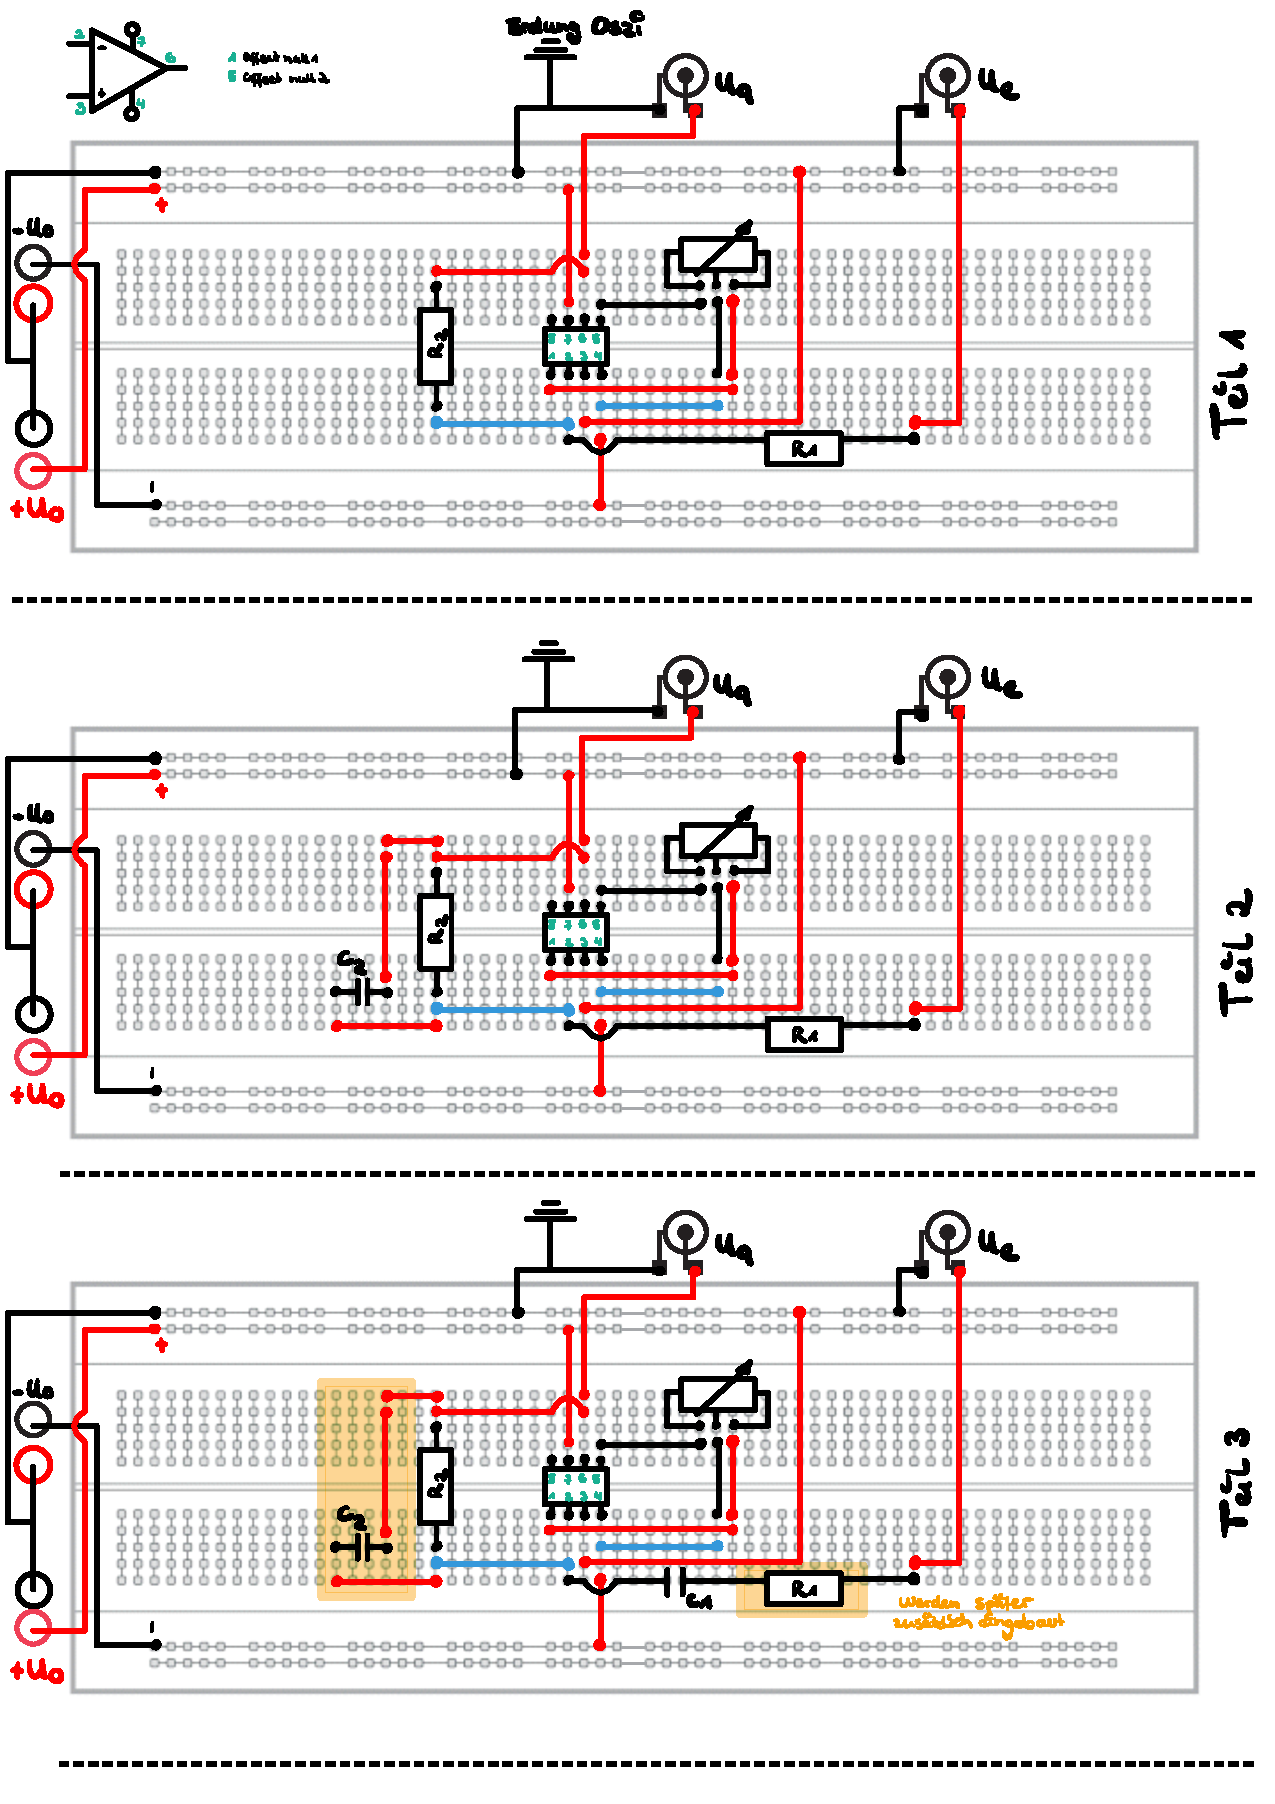
\includepdf[pages = 1, landscape = false, nup = 1x1, scale = \skalierung , pagecommand={}]{30-SteckbretterEL2.pdf}


    % 4.Kapitel Versuchsauswertung
    % Manuel Lippert - Paul Schwanitz
% Physikalisches Praktikum

% 4.Kapitel Versuchsauswertung

\chapter{Auswertung und Diskussion}
\label{chap:versuchsauswertung}

% Text

% Input der Teilauswertung je nach Produktion der Nebendateien ohne Ordner
%Matteo Kumar - Leonhard Schatt
% Fortgeschrittenes Physikalisches Praktikum

% Teilauswertung X

\section{Teilauswertung X}

% etc.

    % 5.Kapitel Fazit
    % 5. Fazit

\chapter{Fazit}
\label{chap:fazit}


% Text

    % Anhang
    %% Matteo Kumar - Leonard Schatt
% Physikalisches Praktikum

% Anhang

\appendix

% Text

% Charlotte Geiger - Manuel Lippert - Leonard Schatt
% Physikalisches Praktikum

% Anhang A

\chapter{Append A}
\label{chap:anhangA}

\section{Teilanhang X}


    % Literatur
    %\bibliographystyle{Auswertung.bst}
    %\nocite{*}
    %\bibliography{Auswertung.bib}

\end{document}